\documentclass[10pt,xcolor={dvipsnames},fleqn]{beamer}
%\documentclass[handout,10pt,xcolor={dvipsnames},fleqn]{beamer}
\usepackage{isse}


\usepackage{apalike}
\usepackage[utf8]{inputenc}
\usepackage{pdfpages}
%\usepackage{ngerman}
\usepackage{stmaryrd,amsmath,amssymb}
\usepackage{color}
\usepackage{enumerate}
\usepackage[makeroom]{cancel}
\usepackage{mdframed}
\usepackage{xskak}
\usepackage{marvosym}
\setchessboard{
showmover=false}
\usepackage[noend]{algpseudocode}   % package for algorithms
\usepackage{algorithm}
\usepackage{tikz}

\usepackage[absolute,overlay]{textpos}

\usetikzlibrary{trees,calc,shapes,arrows,matrix,shadows,decorations.markings}

\mdfdefinestyle{theoremstyle}{
linecolor=red,linewidth=2pt,
frametitlerule=true,
frametitlebackgroundcolor=gray!20,
innertopmargin=\topskip,
}
\definecolor{LRed}{rgb}{1,.8,.8}
\definecolor{MRed}{rgb}{1,.6,.6}
\definecolor{HRed}{rgb}{1,.2,.2}

\usepackage{listings}
\lstdefinelanguage{mzn}
{
	morekeywords={var,int,solve,not,search,satisfy,endif,maximize,minimize,bool,float,constraint,sum,forall,exists,array,of,include,predicate,then,commit,post,set,function,if,else,repeat,next,ann,break},
	sensitive=false,
	morecomment=[l]{\%},
	morecomment=[s]{/*}{*/},
	morestring=[b]",
}

\definecolor{lightlightgray}{gray}{0.95}
\definecolor{forestgreen}{HTML}{009B55}
\definecolor{thermicred}{rgb}{0.82, 0.1, 0.26}
\lstset
{
	basicstyle=\ttfamily\small,
	commentstyle=\ttfamily\color{thermicred},
	stringstyle=\ttfamily\color{isseorange},
	keywordstyle=\ttfamily\color{blue},
	tabsize=2,
	showstringspaces=false,
	flexiblecolumns=true,
	captionpos=b,	
	backgroundcolor=\color{lightlightgray},
	frame=single,
	 xleftmargin=\parindent,
}

\lstset{language=mzn}
\interfootnotelinepenalty=10000

% ====== custom commands

\newcommand{\prosumer}[1]{\ensuremath{\mathtt{#1}}}
% Soft Constraint Example
\newcommand{\constraintName}[1]{\ensuremath{\mathtt{#1}}}
% Biogas Constraints
\newcommand{\biogas}{biogas}
\newcommand{\biogasShort}{bio}
\newcommand{\gasFull}{\ensuremath{\constraintName{gasFull}_\mathtt{\biogasShort}}}
\newcommand{\ecoSweet}{\ensuremath{\constraintName{ecoSweet}_\mathtt{\biogasShort}}}
\newcommand{\onOff}{\ensuremath{\constraintName{onOff}_\mathtt{\biogasShort}}}
% Thermal Plant Constraints
\newcommand{\thermal}{thermal}
\newcommand{\thermalShort}{therm}
\newcommand{\ecoOpt}{\ensuremath{\constraintName{ecoOpt}_\mathtt{\thermalShort}}}
\newcommand{\inertia}{\ensuremath{\constraintName{inertia}_\mathtt{\thermalShort}}}
\newcommand{\ecoGood}{\ensuremath{\constraintName{ecoGood}_\mathtt{\thermalShort}}}
\newcommand{\hLevelThermal}[1]{$H_#1^\mathtt{\thermalShort}$}
% Electric Vehicle
\newcommand{\ev}{EV}
\newcommand{\limitBatteryUsage}{\ensuremath{\constraintName{limitBU}_\mathtt{\ev}}}
\newcommand{\prefBatteryLevel}{\ensuremath{\constraintName{prefBL}_\mathtt{\ev}}}
\newcommand{\earlyBird}{\ensuremath{\constraintName{earlyBird}_\mathtt{\ev}}}
% Organization
\newcommand{\org}{org}
\newcommand{\minMaxViolation}{\ensuremath{\constraintName{violation}_\mathtt{\org}}}
\newcommand{\hLevelOrg}[1]{$H_#1^\mathtt{\org}$}

\newcommand{\Variable}{X}
\newcommand{\LocalVariable}{\widehat{\Variable}}
\newcommand{\Domain}{D}
\newcommand{\Constraint}{C}
\newcommand{\ConstraintRelationship}{\mathcal{R}}

\newcommand{\valuation}{v}
\newcommand{\constraint}[1]{\mathrm{#1}}

\newcommand{\plantconstraint}[3]{  
\ifx#1b \constraint{best}[#3]
\else \ifx#1g \constraint{good}[#3]
\else \ifx#1a \constraint{acc}[#3]
\else \ifx#1d \constraint{diff}
\else \ifx#1l \constraint{low}[#3]
\else \ifx#1h \constraint{high}[#3]
\else \ifx#1o \constraint{org}[#3]
   \else
   \constraint{#1}_{#2}^{#3} 
   
   
\fi \fi \fi \fi \fi \fi \fi}
\usepackage{stmaryrd}

\newcommand{\code}[1]{\normalfont\texttt{\spaceskip=3pt\frenchspacing\def\{{\char123}\def\}{\char125}\def\^{\char94}\def\_{\char95}#1}}
\newcommand{\varit}[1]{{\frenchspacing\ensuremath{\normalfont\textsl{#1}}}}
\newcommand{\macit}[1]{{\frenchspacing\ensuremath{\normalfont\textsf{#1}}}}
\newcommand{\Eta}{\mathrm{H}}
\newcommand{\Mu}{\mathrm{M}}
\newcommand{\Nu}{\mathrm{N}}

\newcommand{\NZ}{\mathbb{N}}
\newcommand{\RZ}{\mathbb{R}}
\newcommand{\RZp}{\RZ_{\geq 0}}
\newcommand{\powerset}{\mathcal{P}}
\newcommand{\limp}{\mathrel{\Rightarrow}}
\newcommand{\compfun}{\mathbin{\circ}}
\newcommand{\isorel}{\mathrel{\cong}}
\newcommand{\restrict}[2]{{#1}\mathnormal{\upharpoonright}{#2}}
\newcommand{\natto}{\mathrel{\dot{\mathnormal{\to}}}}
\let\lbagold\lbag
\let\rbagold\rbag
\def\lbag{\mathopen{\lbagold}}
\def\rbag{\mathclose{\rbagold}}

\DeclareMathOperator{\Minop}{\mathrm{Min}}
\newcommand{\Min}[1]{\Minop^{#1}}
\DeclareMathOperator{\Maxop}{\mathrm{Max}}
\newcommand{\Max}[1]{\Maxop^{#1}}
\DeclareMathOperator{\finsets}{\mathcal{P}_{\mathrm{fin}}}
\DeclareMathOperator{\nefinsets}{\mathcal{P}_{\mathrm{fin}^+}}
%\DeclareMathOperator{\incfinsets}{\mathcal{I}_{\mathrm{fin}}}
\newcommand{\incfinsets}[1]{\mathcal{I}_{\mathrm{fin}}^{#1}}
\newcommand{\lowersubseteq}[1]{\mathrel{\subseteq_{#1}}}
\newcommand{\lowersupseteq}[1]{\mathrel{\supseteq_{#1}}}
\newcommand{\lowersubset}[1]{\mathrel{\subset_{#1}}}
\newcommand{\lowersupset}[1]{\mathrel{\supset_{#1}}}
\newcommand{\uppersubseteq}[1]{\mathrel{\subseteq^{#1}}}
\newcommand{\uppersupseteq}[1]{\mathrel{\supseteq^{#1}}}
\newcommand{\uppersubset}[1]{\mathrel{\subset^{#1}}}
\newcommand{\uppersupset}[1]{\mathrel{\supset^{#1}}}
\newcommand{\lowercup}[1]{\mathbin{\cup_{#1}}}
\newcommand{\uppercup}[1]{\mathbin{\cup^{#1}}}

\DeclareMathOperator{\finmsets}{\mathcal{M}_{\mathrm{fin}}}
\DeclareMathOperator{\nefinmsets}{\mathcal{M}_{\mathrm{fin}^+}}
\newcommand{\mcup}{\mathbin{\mathnormal{\cup}\llap{\text{\fontsize{8pt}{8pt}\selectfont$-$}}}}
\newcommand{\submseteq}{%
\mathrel{\mathchoice%
{\mathnormal{\subseteq}\llap{\text{\raisebox{0.3pt}{\fontsize{8pt}{8pt}\selectfont\rotatebox{90}{$-$}\hspace{1.8pt}}}}}%
{\mathnormal{\subseteq}\llap{\text{\raisebox{0.3pt}{\fontsize{8pt}{8pt}\selectfont\rotatebox{90}{$-$}\hspace{1.8pt}}}}}%
{\mathnormal{\subseteq}\llap{\text{\raisebox{-0.3pt}{\fontsize{5pt}{5pt}\selectfont\rotatebox{90}{$-$}\hspace{1.4pt}}}}}%
{\mathnormal{\subseteq}\llap{\text{\raisebox{-0.3pt}{\fontsize{5pt}{5pt}\selectfont\rotatebox{90}{$-$}\hspace{1.4pt}}}}}%
}}
\newcommand{\supmseteq}{\mathrel{\reflectbox{$\submseteq$}}}
\newcommand{\lowersubmseteq}[1]{\mathrel{\submseteq_{#1}}}
\newcommand{\uppersubmseteq}[1]{\mathrel{\submseteq^{#1}}}
\newcommand{\submset}{%
\mathrel{\mathchoice%
{\mathnormal{\subset}\llap{\text{\raisebox{-0.8pt}{\fontsize{8pt}{8pt}\selectfont\rotatebox{90}{$-$}\hspace{1.8pt}}}}}%
{\mathnormal{\subset}\llap{\text{\raisebox{-0.8pt}{\fontsize{8pt}{8pt}\selectfont\rotatebox{90}{$-$}\hspace{1.8pt}}}}}%
{\mathnormal{\subset}\llap{\text{\raisebox{-0.3pt}{\fontsize{7pt}{7pt}\selectfont\rotatebox{90}{$-$}\hspace{1pt}}}}}%
{\mathnormal{\subset}\llap{\text{\raisebox{-0.3pt}{\fontsize{7pt}{7pt}\selectfont\rotatebox{90}{$-$}\hspace{1pt}}}}}%
}}
\newcommand{\supmset}{\mathrel{\reflectbox{$\submset$}}}
\newcommand{\lowersubmset}[1]{\mathrel{\submset_{#1}}}
\newcommand{\uppersubmset}[1]{\mathrel{\submset^{#1}}}

\DeclareMathOperator{\collapseset}{\mathcal{C}}

\newcommand{\category}[1]{\mathrm{#1}}
\newcommand{\POcat}{\category{PO}}
\newcommand{\uSLcat}{\category{uSL}}
\newcommand{\poMoncat}{\category{poMon}}
\newcommand{\jMoncat}{\category{jMon}}
\newcommand{\mMoncat}{\category{mMon}}
\newcommand{\xMoncat}{{x}\category{Mon}}
\newcommand{\PVScat}{\category{PVS}}
\newcommand{\cSRngcat}{\category{cSRng}}
\newcommand{\DAGcat}{\category{DAG}}

\newcommand{\idfun}[1]{1_{#1}}
\newcommand{\functor}[1]{\mathit{#1}}
\DeclareMathOperator{\POfun}{\functor{PO}}
\DeclareMathOperator{\uSLfun}{\functor{uSL}}
\DeclareMathOperator{\poMonfun}{\functor{poMon}}
\DeclareMathOperator{\jMonfun}{\functor{jMon}}
\DeclareMathOperator{\mMonfun}{\functor{mMon}}
\DeclareMathOperator{\xMonfun}{\text{$x$}\functor{Mon}}
\DeclareMathOperator{\PVSfun}{\functor{PVS}}
\DeclareMathOperator{\cSRngfun}{\functor{cSRng}}
\DeclareMathOperator{\DAGfun}{\functor{DAG}}

\newcommand{\uSLfree}[1]{\uSLfun\langle#1\rangle}
\newcommand{\uSLeta}{\eta^{\uSLcat}}
\newcommand{\uSLetaat}[1]{\uSLeta_{#1}}
\newcommand{\uSLlift}[1]{{#1}^{\sharp_{\uSLcat}}}

\newcommand{\poMonfree}[1]{\poMonfun\langle#1\rangle}
\newcommand{\poMoneta}{\eta^{\poMoncat}}
\newcommand{\poMonetaat}[1]{\poMoneta_{#1}}
\newcommand{\poMonlift}[1]{{#1}^{\sharp_{\poMoncat}}}

\newcommand{\jMonfree}[1]{\jMonfun\langle#1\rangle}
\newcommand{\jMoneta}{\eta^{\jMoncat}}
\newcommand{\jMonetaat}[1]{\jMoneta_{#1}}
\newcommand{\jMonlift}[1]{{#1}^{\sharp_{\jMoncat}}}

\newcommand{\mMonfree}[1]{\mMonfun\langle#1\rangle}
\newcommand{\mMoneta}{\eta^{\mMoncat}}
\newcommand{\mMonetaat}[1]{\mMoneta_{#1}}
\newcommand{\mMonlift}[1]{{#1}^{\sharp_{\mMoncat}}}

\newcommand{\PVSfree}[1]{\PVSfun\langle#1\rangle}
\newcommand{\PVSeta}{\eta^{\PVScat}}
\newcommand{\PVSetaat}[1]{\PVSeta_{#1}}
\newcommand{\PVSlift}[1]{{#1}^{\sharp_{\PVScat}}}

\newcommand{\xMonfree}[1]{\xMonfun\langle#1\rangle}
\newcommand{\xMoneta}{\eta^{\xMoncat}}
\newcommand{\xMonetaat}[1]{\xMoneta_{#1}}
\newcommand{\xMonlift}[1]{{#1}^{\sharp_{\xMoncat}}}

\newcommand{\cSRngfree}[1]{\cSRngfun\langle#1\rangle}
\newcommand{\cSRngeta}{\eta^{\cSRngcat}}
\newcommand{\cSRngetaat}[1]{\cSRngeta_{#1}}
\newcommand{\cSRnglift}[1]{{#1}^{\sharp_{\cSRngcat}}}

\newcommand{\POfree}[1]{\POfun\langle#1\rangle}
\newcommand{\POeta}{\eta^{\POcat}}
\newcommand{\POetaat}[1]{\POeta_{#1}}
\newcommand{\POlift}[1]{{#1}^{\sharp_{\POcat}}}

\newcommand{\mtimes}[1]{\mathbin{\tilde{\cdot}_{#1}}}
\newcommand{\mplus}[1]{\mathbin{\tilde{\cup}_{#1}}}
\newcommand{\ftimes}[1]{\mathbin{\tilde{\mcup}^{#1}}}
\newcommand{\fplus}[1]{\mathbin{\tilde{\cup}_{#1}}}

\DeclareMathOperator{\scope}{\mathrm{sc}}
\DeclareMathOperator{\defdom}{\mathrm{def}}

\newcommand{\reflclos}[1]{\mathrel{(#1)^=}}
\newcommand{\transclos}[2][+]{\mathrel{(#2)^{#1}}}
\newcommand{\refltransclos}[1]{\mathrel{(#1)^*}}

\newcommand{\XPDrel}[2][\pi]{\rightsquigarrow^{#1}_{#2}}
\newcommand{\XPDreleq}[2][\pi]{\rightsquigarrow^{#1, =}_{#2}}
\newcommand{\XPDord}[2][\pi]{<^{#1}_{#2}}
\newcommand{\XPDordeq}[2][\pi]{\geq^{#1}_{#2}}
\newcommand{\XPDleq}[2][\pi]{\leq^{#1}_{#2}}
\newcommand{\XPDgeq}[2][\pi]{\geq^{#1}_{#2}}
\newcommand{\XPDw}[2][\pi]{w^{#1}_{#2}}
\newcommand{\XPDW}[2][\pi]{W^{#1}_{#2}}
\newcommand{\XPDk}[2][\pi]{k^{#1}_{#2}}

\newcommand{\SPDrel}{\XPDrel[\mathrm{SPD}]}
\newcommand{\SPDreleq}{\XPDreleq[\mathrm{SPD}]}
\newcommand{\SPDleq}{\XPDleq[\mathrm{SPD}]}
\newcommand{\SPDgeq}{\XPDgeq[\mathrm{SPD}]}
\newcommand{\SPDord}{\XPDord[\mathrm{SPD}]}
\newcommand{\SPDw}{\XPDw[\mathrm{SPD}]}
\newcommand{\SPDW}{\XPDW[\mathrm{SPD}]}
\newcommand{\DPDrel}{\XPDrel[\mathrm{DPD}]}
\newcommand{\DPDreleq}{\XPDreleq[\mathrm{DPD}]}
\newcommand{\DPDord}{\XPDord[\mathrm{DPD}]}
\newcommand{\DPDw}{\XPDw[\mathrm{DPD}]}
\newcommand{\DPDW}{\XPDW[\mathrm{DPD}]}
\newcommand{\TPDrel}{\XPDrel[\mathrm{TPD}]}
\newcommand{\TPDreleq}{\XPDreleq[\mathrm{TPD}]}
\newcommand{\TPDleq}{\XPDleq[\mathrm{TPD}]}
\newcommand{\TPDgeq}{\XPDgeq[\mathrm{TPD}]}
\newcommand{\TPDord}{\XPDord[\mathrm{TPD}]}
\newcommand{\TPDw}{\XPDw[\mathrm{TPD}]}
\newcommand{\TPDW}{\XPDW[\mathrm{TPD}]}

\DeclareMathSymbol{\UPi}{\mathalpha}{operators}{"05}



\renewcommand{\submseteq}{%
\mathrel{\mathchoice%
{\mathnormal{\subseteq}\llap{\text{\raisebox{0.0pt}{\fontsize{7.5pt}{7.5pt}\selectfont\rotatebox{90}{$-$}\hspace{1.6pt}}}}}%
{\mathnormal{\subseteq}\llap{\text{\raisebox{0.0pt}{\fontsize{7.5pt}{7.5pt}\selectfont\rotatebox{90}{$-$}\hspace{1.6pt}}}}}%
{\mathnormal{\subseteq}\llap{\text{\raisebox{-0.3pt}{\fontsize{7pt}{7pt}\selectfont\rotatebox{90}{$-$}\hspace{1pt}}}}}%
{\mathnormal{\subseteq}\llap{\text{\raisebox{-0.3pt}{\fontsize{7pt}{7pt}\selectfont\rotatebox{90}{$-$}\hspace{1pt}}}}}%
}}


\tikzset{
   main node/.style={circle,fill=black!15,draw,font=\sffamily},
   constraint node/.style={main node, circle, inner sep=2pt,font=\sffamily\small},   
   treestyle/.style={rectangle,fill=black!15,draw,font=\sffamily}
}


\mdtheorem[style=theoremstyle]{definition}{Definition}

\renewcommand{\vec}[1]{\mathbf{#1}}
\newcommand{\tupleOf}[1]{\langle #1 \rangle}
\newcommand{\cemph}[1]{\alert{#1}}
\usepackage{framed}
\usepackage{ifthen}

\usetikzlibrary{decorations.pathmorphing,calc,shadows.blur,shadings}
\usetikzlibrary{mindmap,trees,automata,arrows}
\usepackage{extrabeamercmds}

\newcommand{\hFirst}[1]{{\color{isseorange} #1}}
\newcommand{\hSecond}[1]{{\color{issegrey} #1}}

\newcounter{mathseed}
\setcounter{mathseed}{3}
\pgfmathsetseed{\arabic{mathseed}} % To have predictable results
% Define a background layer, in which the parchment shape is drawn
\pgfdeclarelayer{background}
\pgfsetlayers{background,main}


% This is the base for the fractal decoration. It takes a random point between the start and end, and
% raises it a random amount, thus transforming a segment into two, connected at that raised point
% This decoration can be applied again to each one of the resulting segments and so on, in a similar
% way of a Koch snowflake.
\pgfdeclaredecoration{irregular fractal line}{init}
{
  \state{init}[width=\pgfdecoratedinputsegmentremainingdistance]
  {
    \pgfpathlineto{\pgfpoint{random*\pgfdecoratedinputsegmentremainingdistance}{(random*\pgfdecorationsegmentamplitude-0.02)*\pgfdecoratedinputsegmentremainingdistance}}
    \pgfpathlineto{\pgfpoint{\pgfdecoratedinputsegmentremainingdistance}{0pt}}
  }
}


% define some styles
\tikzset{
   paper/.style={draw=black!10, blur shadow, every shadow/.style={opacity=1, black}, 
                 lower left=black!10, upper left=black!5, upper right=white, lower right=black!5, fill=none},
   irregular cloudy border/.style={decoration={irregular fractal line, amplitude=0.2},
           decorate,
     },
   irregular spiky border/.style={decoration={irregular fractal line, amplitude=-0.2},
           decorate,
     },
   ragged border/.style={ decoration={random steps, segment length=7mm, amplitude=2mm},
           decorate,
   }
}

\tikzset{
  normal border/.style={orange!30!black!10, decorate, 
     decoration={random steps, segment length=2.5cm, amplitude=.7mm}},
  torn border/.style={orange!30!black!5, decorate, 
     decoration={random steps, segment length=.5cm, amplitude=1.7mm}}}


\def\tornpaper#1{%
\ifthenelse{\isodd{\value{mathseed}}}{%
\tikz{
  \node[inner sep=1em] (A) {#1};  % Draw the text of the node
  \begin{pgfonlayer}{background}  % Draw the shape behind
  \fill[paper] % recursively decorate the bottom border
     \pgfextra{\pgfmathsetseed{\arabic{mathseed}}\addtocounter{mathseed}{1}}%
      {decorate[irregular cloudy border]{decorate{decorate{decorate{decorate[ragged border]{
        (A.north west) -- (A.north east)
      }}}}}}
      -- (A.south east)
     \pgfextra{\pgfmathsetseed{\arabic{mathseed}}}%
      {decorate[irregular spiky border]{decorate{decorate{decorate{decorate[ragged border]{
      -- (A.south west)
      }}}}}}
      -- (A.north west);
  \end{pgfonlayer}}
}{%
\tikz{
  \node[inner sep=1em] (A) {#1};  % Draw the text of the node
  \begin{pgfonlayer}{background}  % Draw the shape behind
  \fill[paper] % recursively decorate the bottom border
     \pgfextra{\pgfmathsetseed{\arabic{mathseed}}\addtocounter{mathseed}{1}}%
      {decorate[irregular spiky border]{decorate{decorate{decorate{decorate[ragged border]{
        (A.north east) -- (A.north west)
      }}}}}}
      -- (A.south west)
     \pgfextra{\pgfmathsetseed{\arabic{mathseed}}}%
      {decorate[irregular cloudy border]{decorate{decorate{decorate{decorate[ragged border]{
      -- (A.south east)
      }}}}}}
      -- (A.north east);
  \end{pgfonlayer}}
}}


% Macro to draw the shape behind the text, when it fits completly in the
% page
\def\parchmentframe#1{
\tikz{
  \node[inner sep=2em] (A) {#1};  % Draw the text of the node
  \begin{pgfonlayer}{background}  % Draw the shape behind
  \fill[normal border] 
        (A.south east) -- (A.south west) -- 
        (A.north west) -- (A.north east) -- cycle;
  \end{pgfonlayer}}}

% Macro to draw the shape, when the text will continue in next page
\def\parchmentframetop#1{
\tikz{
  \node[inner sep=2em] (A) {#1};    % Draw the text of the node
  \begin{pgfonlayer}{background}    
  \fill[normal border]              % Draw the ``complete shape'' behind
        (A.south east) -- (A.south west) -- 
        (A.north west) -- (A.north east) -- cycle;
  \fill[torn border]                % Add the torn lower border
        ($(A.south east)-(0,.2)$) -- ($(A.south west)-(0,.2)$) -- 
        ($(A.south west)+(0,.2)$) -- ($(A.south east)+(0,.2)$) -- cycle;
  \end{pgfonlayer}}}

% Macro to draw the shape, when the text continues from previous page
\def\parchmentframebottom#1{
\tikz{
  \node[inner sep=2em] (A) {#1};   % Draw the text of the node
  \begin{pgfonlayer}{background}   
  \fill[normal border]             % Draw the ``complete shape'' behind
        (A.south east) -- (A.south west) -- 
        (A.north west) -- (A.north east) -- cycle;
  \fill[torn border]               % Add the torn upper border
        ($(A.north east)-(0,.2)$) -- ($(A.north west)-(0,.2)$) -- 
        ($(A.north west)+(0,.2)$) -- ($(A.north east)+(0,.2)$) -- cycle;
  \end{pgfonlayer}}}

% Macro to draw the shape, when both the text continues from previous page
% and it will continue in next page
\def\parchmentframemiddle#1{
\tikz{
  \node[inner sep=2em] (A) {#1};   % Draw the text of the node
  \begin{pgfonlayer}{background}   
  \fill[normal border]             % Draw the ``complete shape'' behind
        (A.south east) -- (A.south west) -- 
        (A.north west) -- (A.north east) -- cycle;
  \fill[torn border]               % Add the torn lower border
        ($(A.south east)-(0,.2)$) -- ($(A.south west)-(0,.2)$) -- 
        ($(A.south west)+(0,.2)$) -- ($(A.south east)+(0,.2)$) -- cycle;
  \fill[torn border]               % Add the torn upper border
        ($(A.north east)-(0,.2)$) -- ($(A.north west)-(0,.2)$) -- 
        ($(A.north west)+(0,.2)$) -- ($(A.north east)+(0,.2)$) -- cycle;
  \end{pgfonlayer}}}

% Define the environment which puts the frame
% In this case, the environment also accepts an argument with an optional
% title (which defaults to ``Example'', which is typeset in a box overlaid
% on the top border
\newenvironment{parchment}[1][Example]{%
  \def\FrameCommand{\parchmentframe}%
  \def\FirstFrameCommand{\parchmentframetop}%
  \def\LastFrameCommand{\parchmentframebottom}%
  \def\MidFrameCommand{\parchmentframemiddle}%
  \vskip\baselineskip
  \MakeFramed {\FrameRestore}
  \noindent\tikz\node[inner sep=1ex, draw=black!20,fill=white, 
          anchor=west, overlay] at (0em, 2em) {\sffamily#1};\par}%
{\endMakeFramed}


\title{Constraint Relationships}
\author{Step-by-Step Enhancing a MiniZinc Model}

\date{\today}

\begin{document}

\titleframe

%\begin{frame}
%\frametitle{Preferences in Constraint Solving}
%
%Constraint problem $(X, D, C)$ 
%\begin{itemize}
%  \item \cemph{Variables} $X$,
%\cemph{Domains} $D = (D_x)_{x \in X}$,
%\cemph{Constraints} $C$
%\end{itemize}
%
%\vspace*{1ex}
%
%How to deal with \cemph{over-constrained} problems?
%
%\vspace*{2ex}
%
%$((\{ \mathrm{x}, \mathrm{y}, \mathrm{z} \},
%\mathrm{D}_{\mathrm{x}} = \mathrm{D}_{\mathrm{y}} =
%\mathrm{D}_{\mathrm{z}} = \{ 1, 2, 3 \}), \{ \mathrm{c}_1,
%\mathrm{c}_2, \mathrm{c}_3 \})$ mit 
%\bgroup\abovedisplayskip4pt\belowdisplayskip4pt
%\begin{align*}
%  \mathrm{c}_1 &: \mathrm{x} + 1 = \mathrm{y}
%\\[-.4ex]
%  \mathrm{c}_2 &: \mathrm{z} = \mathrm{y} + 2
%\\[-.4ex]
%  \mathrm{c}_3 &: \mathrm{x} + \mathrm{y} \leq 3
%\end{align*}
%\egroup
%
%\begin{itemize}
%  \item Not all constraints can be satisfied simultaneously
%\begin{itemize} 
%  \item e.\,g., $\mathrm{c}_2$ forces $\mathrm{z} = 3$ and $\mathrm{y} = 1$, conflicting $\mathrm{c}_1$
%\end{itemize}
%
%  \item We can \cemph{choose} between assignments satisfying $\{ \mathrm{c}_1, \mathrm{c}_3 \}$ or $\{ \mathrm{c}_2, \mathrm{c}_3 \}$.
%\end{itemize}
%
%\vspace*{2ex}
%
%Which assignments $v \in [X \to D]$ should be \alert{preferred} by an agent/several agents?
%
%\end{frame}
%
%\begin{frame}
%\frametitle{Constraint Relationships}
%
%Approach~\cite{Schiendorfer13}
%\begin{itemize}
%  \item Define relation $R$ over constraints $C$ to denote which constraints are more important than others, e.\,g.
%\begin{itemize}
%  \item $\mathrm{c}_1$ is more important than  $\mathrm{c}_2$
%
%  \item $\mathrm{c}_1$ is more important than $\mathrm{c}_3$
%\end{itemize}
%\end{itemize}
%\begin{textblock*}{2.5cm}[1,1](\textwidth-1.5cm,\textheight-4.03cm)
%\begin{tikzpicture}[auto,
%                    ->,>=stealth',shorten >=1pt,thick,
%                    node distance=.7cm,inner sep=2pt,
%                    constraint/.style={circle,fill=black!15,draw,font=\sffamily\small}]
%\node[constraint node] (1) at (0, 0)                   {$\mathrm{c}_1$};
%\node[constraint node] (2) at ($ (1) + (-0.8, -0.8) $) {$\mathrm{c}_2$};  
%\node[constraint node] (3) at ($ (1) + ( 0.8, -0.8) $) {$\mathrm{c}_3$};  
%%  
%\path[every node/.style={font=\sffamily\tiny}]
%  (2) edge (1)
%  (3) edge (1)
%  ;
%\end{tikzpicture}
%\end{textblock*}
%
%\vspace*{5.6ex}
%
%Benefits
%\begin{itemize}
%  \item \cemph{Qualitative} formalism --- easy to specify
%  \item Graphical interpretation 
%\begin{itemize}
% \item Semantics (\alert{how} much more important is a constraint) regulated by 
%  \item \cemph{dominance properties} that are either ``hierarchical'' or ``egalitarian''
%  \item Single-Predecessors-Dominance (SPD) vs. Transitive-Predecessors-Dominance (TPD)
%\end{itemize}
%\end{itemize}
%\end{frame}

\begin{frame}{Synopsis}

\vspace*{2ex}
We will \ldots
\begin{itemize}
\item start with an \alert{n-queens model} in MiniZinc
\item add some additional soft constraints (e.g. one queen should be placed in the \alert{center})
\item prioritize these soft constraints using \alert{constraint relationships}
\item switch dominance properties (SPD, TPD) 
\item and \alert{solve} with: Branch-and-Bound (BaB), Large Neighborhood Search (LNS)
\end{itemize}

\vspace*{2ex}

\url{http://isse-augsburg.github.io/constraint-relationships/}
\end{frame}

\begin{frame}[fragile]{Satisfaction Model}
\lstinputlisting{model-evolution/soft-queens-0.mzn}
\small
\begin{verbatim}
queens = array1d(1..8 ,[4, 6, 1, 5, 2, 8, 3, 7]);
----------
\end{verbatim}
\copyright~Hakan Kjellerstrand, \url{http://www.hakank.org/minizinc}
\end{frame}

\begin{frame}[fragile]{Step 1: Add Soft Constraint Support}
\lstinputlisting{model-evolution/soft-queens-1.mzn}

\begin{itemize}
\item Adds \texttt{nScs} (a new parameter) boolean variables, one for each soft constraint
\item Adds parameter \texttt{penalties} (use \texttt{[1 | i in 1..nScs]} if not relevant)
\item Intuition: The cost of violating soft constraint $\mathtt{i}$ should be \texttt{penalties[i]} 
\end{itemize}
%\small
%\begin{verbatim}
%queens = array1d(1..8 ,[4, 6, 1, 5, 2, 8, 3, 7]);
%----------
%\end{verbatim}
\end{frame}

\begin{frame}[fragile]{Step 1: Behind the Scenes}

\begin{lstlisting}
include "link_set_to_booleans.mzn";
% MODEL-SPECIFIC parameters: nScs and penalties
int: nScs; set of int: SOFTCONSTRAINTS = 1..nScs;

% reified variables for each soft constraint
array[SOFTCONSTRAINTS] of var bool: satisfied;
array[SOFTCONSTRAINTS] of var bool: violated = 
   [not satisfied[sc] | sc in SOFTCONSTRAINTS] ;

array[SOFTCONSTRAINTS] of int: penalties;
var int: penSum = sum(sc in SOFTCONSTRAINTS)
   (bool2int(not satisfied[sc]) * penalties[sc]);

var set of SOFTCONSTRAINTS: violatedScs;
constraint link_set_to_booleans(violatedScs,violated); 
\end{lstlisting}
\begin{itemize}
\item Using \texttt{satisfied} \emph{and} \texttt{violated} is done for convenience in expressing 
soft constraints
\item There is also a variant without \texttt{violatedScs} for solvers that do not
support set variables (e.g. MIP): \texttt{soft\_constraints\_noset.mzn} 
\end{itemize}
%\small
%\begin{verbatim}
%queens = array1d(1..8 ,[4, 6, 1, 5, 2, 8, 3, 7]);
%----------
%\end{verbatim}
\end{frame}

\begin{frame}[fragile]{Step 1: Behind the Scenes}

\begin{lstlisting}
% find the sorted permutation of soft constraint instances
array[SOFTCONSTRAINTS] of SOFTCONSTRAINTS: sortPermScs = 
  arg_sort(penalties);
% invert, since arg_sort use <= and we need decreasing order
array[SOFTCONSTRAINTS] of SOFTCONSTRAINTS: mostImpFirst = 
  [ sortPermScs[nScs-s+1] | s in SOFTCONSTRAINTS]; 
\end{lstlisting}
\begin{itemize}
\item \texttt{mostImpFirst} gives an array of soft constraint indices in decreasing order (start with most important ones)
\item Used later as a (generic) labeling strategy
\end{itemize}
%\small
%\begin{verbatim}
%queens = array1d(1..8 ,[4, 6, 1, 5, 2, 8, 3, 7]);
%----------
%\end{verbatim}
\end{frame}

\begin{frame}[fragile]{Step 2: Add Soft Constraints}
\lstinputlisting{model-evolution/soft-queens-2.mzn}

\begin{itemize}
\item Just tie reified soft constraint variables to actual soft constraints
\item \texttt{[1 | i in 1..nScs]} makes it a Max-CSP when minimizing \texttt{penSum}
\end{itemize}
%\small
%\begin{verbatim}
%queens = array1d(1..8 ,[4, 6, 1, 5, 2, 8, 3, 7]);
%----------
%\end{verbatim}
\end{frame}

\begin{frame}[fragile]{Step 2: What about Globals?}
What if want to use global constraints as soft constraints? 
Consider (\texttt{reified.mzn}):
\lstinputlisting{model-evolution/reified.mzn}
Solved with Gecode:
\small
\begin{verbatim}
MiniZinc: flattening error: 'increasing_int' is used in a reified 
context but no reified version is available
\end{verbatim}
\end{frame}

\begin{frame}[fragile]{Step 2: What about Globals?}
\begin{enumerate}
\item[a)] Use a solver that has the reified global, e.g., here: 
\begin{itemize}
\item G12-FD
\item JaCoP
\end{itemize}
\item[b)] Use a decomposition from the MiniZinc standard library (\texttt{reified\_fix.mzn})

\lstinputlisting{model-evolution/reified_fix.mzn}
\end{enumerate}
\end{frame}

\begin{frame}[fragile]{Step 2: What about Globals?}

Solved \texttt{reified\_fix.mzn} with Gecode (same as \texttt{reified.mzn} solved with  JaCoP or G12-FD):
\small

\vspace*{2ex}

\begin{verbatim}
satisfied[1] = false, x = [4, 1, 3, 0, 2]
----------
satisfied[1] = true, x = [0, 1, 2, 3, 4]
----------
==========
\end{verbatim}

\vspace*{2ex}

\normalsize
We do not get the performance benefits of globals (in a decomposition) but at least their conciseness.
\end{frame}

\begin{frame}[fragile]{Step 3: Prioritize Soft Constraints (Weights)}
\lstinputlisting{model-evolution/soft-queens-3w.mzn}

\begin{itemize}
\item If you manually set weights, just add them
\item Switch from \texttt{[1 | i in 1..nScs]} to \texttt{[2, 1, 1]}
\end{itemize}
%\small
%\begin{verbatim}
%queens = array1d(1..8 ,[4, 6, 1, 5, 2, 8, 3, 7]);
%----------
%\end{verbatim}
\end{frame}

\begin{frame}[fragile]{Step 3: Prioritize Soft Constraints (Relations)}
\lstinputlisting{model-evolution/soft-queens-3cr.mzn}

%\small
%\begin{verbatim}
%queens = array1d(1..8 ,[4, 6, 1, 5, 2, 8, 3, 7]);
%----------
%\end{verbatim}
\end{frame}

\begin{frame}[fragile]{Step 3: Prioritize Soft Constraints (Relations)}
\begin{lstlisting}
include "soft_constraints/cr_types.mzn"; % graph types
[... inside cr_types.mzn]
% constraint-relationship-types
int: nCrEdges;
array[1..nCrEdges, 1..2] of SOFTCONSTRAINTS: crEdges;
\end{lstlisting}
Concrete instantiation
\lstinputlisting{model-evolution/cr-soft-queens.dzn}
\begin{center}
%\begin{textblock*}{2.5cm}[1,1](\textwidth-1.5cm,\textheight-4.03cm)
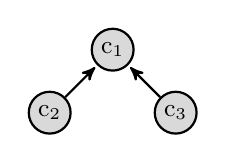
\begin{tikzpicture}[auto,
                    ->,>=stealth',shorten >=1pt,thick,
                    node distance=.7cm,inner sep=2pt,
                    constraint/.style={circle,fill=black!15,draw,font=\sffamily\small}]
\node[constraint node] (1) at (0, 0)                   {$\mathrm{c}_1$};
\node[constraint node] (2) at ($ (1) + (-0.8, -0.8) $) {$\mathrm{c}_2$};  
\node[constraint node] (3) at ($ (1) + ( 0.8, -0.8) $) {$\mathrm{c}_3$};  
%  
\path[every node/.style={font=\sffamily\tiny}]
  (2) edge (1)
  (3) edge (1)
  ;
\end{tikzpicture}
%\end{textblock*}
\end{center}
%\small
%\begin{verbatim}
%queens = array1d(1..8 ,[4, 6, 1, 5, 2, 8, 3, 7]);
%----------
%\end{verbatim}
\end{frame}


\begin{frame}[fragile]{Step 3: Prioritize Soft Constraints (Relations)}
\begin{lstlisting}
include "soft_constraints/cr_weighting.mzn"; % graph types
[... inside cr_weighting.mzn]
function int: weighting(int: s, set of int: softConstraints,
                        array[int, 1..2] of int: edges,
                        bool: useSPD); 
% weigh each constraint higher than the largest child
function int: weightingSPD(int: s, set of int: softConstraints, 
                           array[int] of set of int: dominees) = (
1 + max(s_ in dominees[s])(weightingSPD(s_, softConstraints, dominees));

\end{lstlisting}
\begin{lstlisting}
% weighting(s, SOFTCONSTRAINTS, crEdges, true) 
[2, 1, 1]
% weighting(s, SOFTCONSTRAINTS, crEdges, false) more than chi. together
[3, 1, 1]
\end{lstlisting}
\begin{center}
%\begin{textblock*}{2.5cm}[1,1](\textwidth-1.5cm,\textheight-4.03cm)
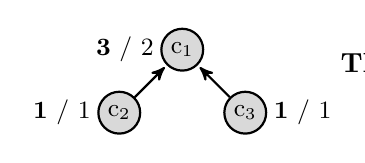
\begin{tikzpicture}[auto,
                    ->,>=stealth',shorten >=1pt,thick,
                    node distance=.7cm,inner sep=2pt,
                    constraint/.style={circle,fill=black!15,draw,font=\sffamily\small}]
\node[constraint node,label=west:{\small \textbf{3} / 2}] (1) at (0, 0)                   {$\mathrm{c}_1$};
\node[constraint node,label=west:{\small \textbf{1} / 1}] (2) at ($ (1) + (-0.8, -0.8) $) {$\mathrm{c}_2$};  
\node[constraint node,label=east:{\small \textbf{1} / 1}] (3) at ($ (1) + ( 0.8, -0.8) $) {$\mathrm{c}_3$};  
\node[overlay](legend) at (3,-0.2) {\textbf{TPD} / SPD} ;
%  
\path[every node/.style={font=\sffamily\tiny}]
  (2) edge (1)
  (3) edge (1)
  ;
\end{tikzpicture}
%\end{textblock*}
\end{center}
%\small
%\begin{verbatim}
%queens = array1d(1..8 ,[4, 6, 1, 5, 2, 8, 3, 7]);
%----------
%\end{verbatim}
\end{frame}

\begin{frame}[fragile]{Step 4: Switch to PVS Architecture}
\lstinputlisting{model-evolution/soft-queens-4.mzn}
\small
\begin{itemize}
\item Defines \emph{single-predecessor-dominance} as solution ordering with predicate
\texttt{spd\_worse}
\item Hides the weight calculation in \texttt{pvs\_spd.mzn}
\end{itemize}
%\small
%\begin{verbatim}
%queens = array1d(1..8 ,[4, 6, 1, 5, 2, 8, 3, 7]);
%----------
%\end{verbatim}
\end{frame}

\begin{frame}[fragile]{Step 4: Switch to PVS Architecture}
\textbf{Idea} Many soft constraint formalisms are generalized by \alert{partial valuation structures}~\cite{Gadducci2013} that
give the codomain of the objective function an \emph{algebraic structure}.
\begin{itemize}
\item A partially ordered valuation structure is described by $(M, \oplus_M, \leq_M, \varepsilon_M)$ where 
\begin{itemize}
\item $M$ \ldots is a set of violation/satisfaction degrees, e.g., $\mathbb{N}$ for weights, $[0,1]$ for probabilities etc.
\item $\oplus_M$ \ldots is a binary \emph{combination} operation to aggregate values from $M$, e.g., $3 \oplus_M  5 \equiv 3 + 5$
\item $\leq_M$ \ldots is a partial \emph{order} over $M$ operation to rank values from $M$, e.g., $5 \leq_M  3 \equiv 5 \geq 3$, $m \leq_M n$ means $m$ \emph{is worse} than $n$
\item $m \leq_M \varepsilon_M$ \ldots for every $m \in M$, i.e. $\varepsilon_M$ is the \emph{best} possible solution, e.g. $0$ violation 
\end{itemize}
\item Similar~\cite{Bistarelli1999}: c-semirings and (total) valuation structures (\texttt{toulbar2})
\end{itemize}
%\small
%\begin{verbatim}
%queens = array1d(1..8 ,[4, 6, 1, 5, 2, 8, 3, 7]);
%----------
%\end{verbatim}
\end{frame}

\begin{frame}[fragile]{Step 4: Switch to PVS Architecture}
\begin{center}
\begin{tabular}{l|c|c|c|c}
\textbf{Concrete PVS} & $M$ & $\oplus_M$ & $\leq_M$ & $\varepsilon_M$ \\ 
\hline 
Weighted CSP & $\mathbb{N}$ & $+$ & $\geq$ & $0$ \\ 
Fuzzy CSP & $[0,1]$ & $\min$ & $\leq$  & 1 \\ 
Constraint Relationships\footnote{$C_s$ is the set of soft constraints, $\subseteq_{\mathsf{SPD}}$ is the SPD-ordering on sets.} &$2^{C_s}$ & $\cup$ & $\subseteq_{\mathsf{SPD}}$ & $\emptyset$ \\ 
\end{tabular} 
\end{center}

\begin{parchment}[Main Idea]
Implement search strategies (BaB and LNS) for partially ordered valuation structures. Instantiate for concrete problems.
\end{parchment}
\alert{From now on we rely on MiniSearch (\url{www.minizinc.org/minisearch/}).}
\end{frame}

\begin{frame}[fragile]{Step 5: Use PVS-based Search}
\lstinputlisting{model-evolution/soft-queens-5.mzn}
\small
\begin{verbatim}
minisearch soft-queens-5.mzn cr-soft-queens.dzn 
\end{verbatim}
\end{frame}

\begin{frame}[fragile]{Step 5: Use PVS-based Search}
\begin{lstlisting}
% only declare predicate for worsening
predicate isWorse(var set of int: leftViolatedScs, 
                    var set of int: rightViolatedScs); 
function ann: strictlyBetterBAB(var set of SOFTCONSTRAINTS: violatedScs) 
=      repeat(
           if next() then 
               let { set of SOFTCONSTRAINTS: lb = sol(violatedScs);} in (
                 print("Intermediate solution:") /\ print() /\
                 commit() /\ post(isWorse(lb, violatedScs))
               )
           else break endif);
\end{lstlisting}
\small
Only relies on \texttt{isWorse}!

\begin{lstlisting}
[... inside pvs_spd.mzn]
predicate isWorse(var set of int: leftViolatedScs, 
                  var set of int: rightViolatedScs) = (
  spd_worse(leftViolatedScs, rightViolatedScs, SOFTCONSTRAINTS, crEdges)
);

\end{lstlisting}
\end{frame}

\begin{frame}[fragile]{Step 5: Use PVS-based Search}
Similar for large neighborhood search
\begin{lstlisting}
% adapted from lns_max an objective value 
function ann: lns_pvs (var set of SOFTCONSTRAINTS: violatedScs, 
                      array[int] of var int: x,
                   int: iterations, float: d) = 
    repeat (i in 1..iterations) (
        scope(
            post(neighbourhoodCts(x,d)) /\ next() /\ commit() /\ 
            print("Intermediate solution: \(sol(violatedScs))\n") /\
            print()
        ) /\
        let { set of SOFTCONSTRAINTS: lb = sol(violatedScs); } in 
        ( post(
           isWorse(lb, violatedScs) 
          ) 
        )
   );

\end{lstlisting}
\small
Only relies on \texttt{isWorse}!

\end{frame}

\begin{frame}{Summary}
This concludes our little transition guide to enhance a MiniZinc model


\vspace*{2ex}

Make sure to check out our other slides about:
\begin{itemize}
\item Language features (more insight about the search strategies and consistency helpers)
\item Case Studies (for some specific examples)
\end{itemize}

\vspace*{2ex}

\url{http://isse-augsburg.github.io/constraint-relationships/}
\end{frame}


\begin{frame}[allowframebreaks]
        \frametitle{Quellen}
        \bibliographystyle{apalike}
        \bibliography{references.bib}
\end{frame}


\end{document}

